\documentclass[12pt,a4paper]{report}
\usepackage{cite}
\usepackage{longtable}
\usepackage[dvips]{graphicx,color}
\usepackage{makeidx}
\usepackage{nomencl}
\usepackage{float}
\usepackage{amsmath}
\usepackage{graphicx}
\usepackage{amssymb}
\usepackage{multicol}
\usepackage{dsfont}
\usepackage[bottom]{footmisc}
\usepackage{subfigure}
\usepackage[OT2,OT1]{fontenc}
\newcommand{\imsize}{3in}
\renewcommand{\bibname}{References}
\newcommand{\norm}[1]{\left|\left|#1\right|\right|}
\newtheorem{definition}{Definition}
\newtheorem {remark}{Remark}
\newtheorem{thm}{Theorem}
\setlength{\textwidth}{6.3in}
\setlength{\textheight}{8.8in}
\addtolength{\oddsidemargin}{-0.5in}
\addtolength{\topmargin}{-0.2in}
\usepackage{tikz}
\usetikzlibrary{shapes,arrows,chains,matrix,positioning,scopes,decorations.pathmorphing,shadows,calc}

\begin{document}
\title{
	\textbf
	{\LARGE{IMPEDANCE-BASED BATTERY MANAGEMENT SYSTEM FOR SAFETY MONITORING OF LITHIUM-ION BATTERIES}} \vspace{.2in} \\ 
	}
\author{
	{\Large{Seminar Report}} \\
	{\large{Seventh semester}} \\
	{\large{Bachelor of Technology}}\vspace{.25in}\\
	{\bf\large ALIN ANTO} \\
	Student \\
	Roll No : TCR15EE016 \vspace{0.25in} \\
	Under the Guidance of \\
	{\bf Prof. Uma Syamkumar} \\
	{\bf Dr. Ramesh Kumar P} \\
	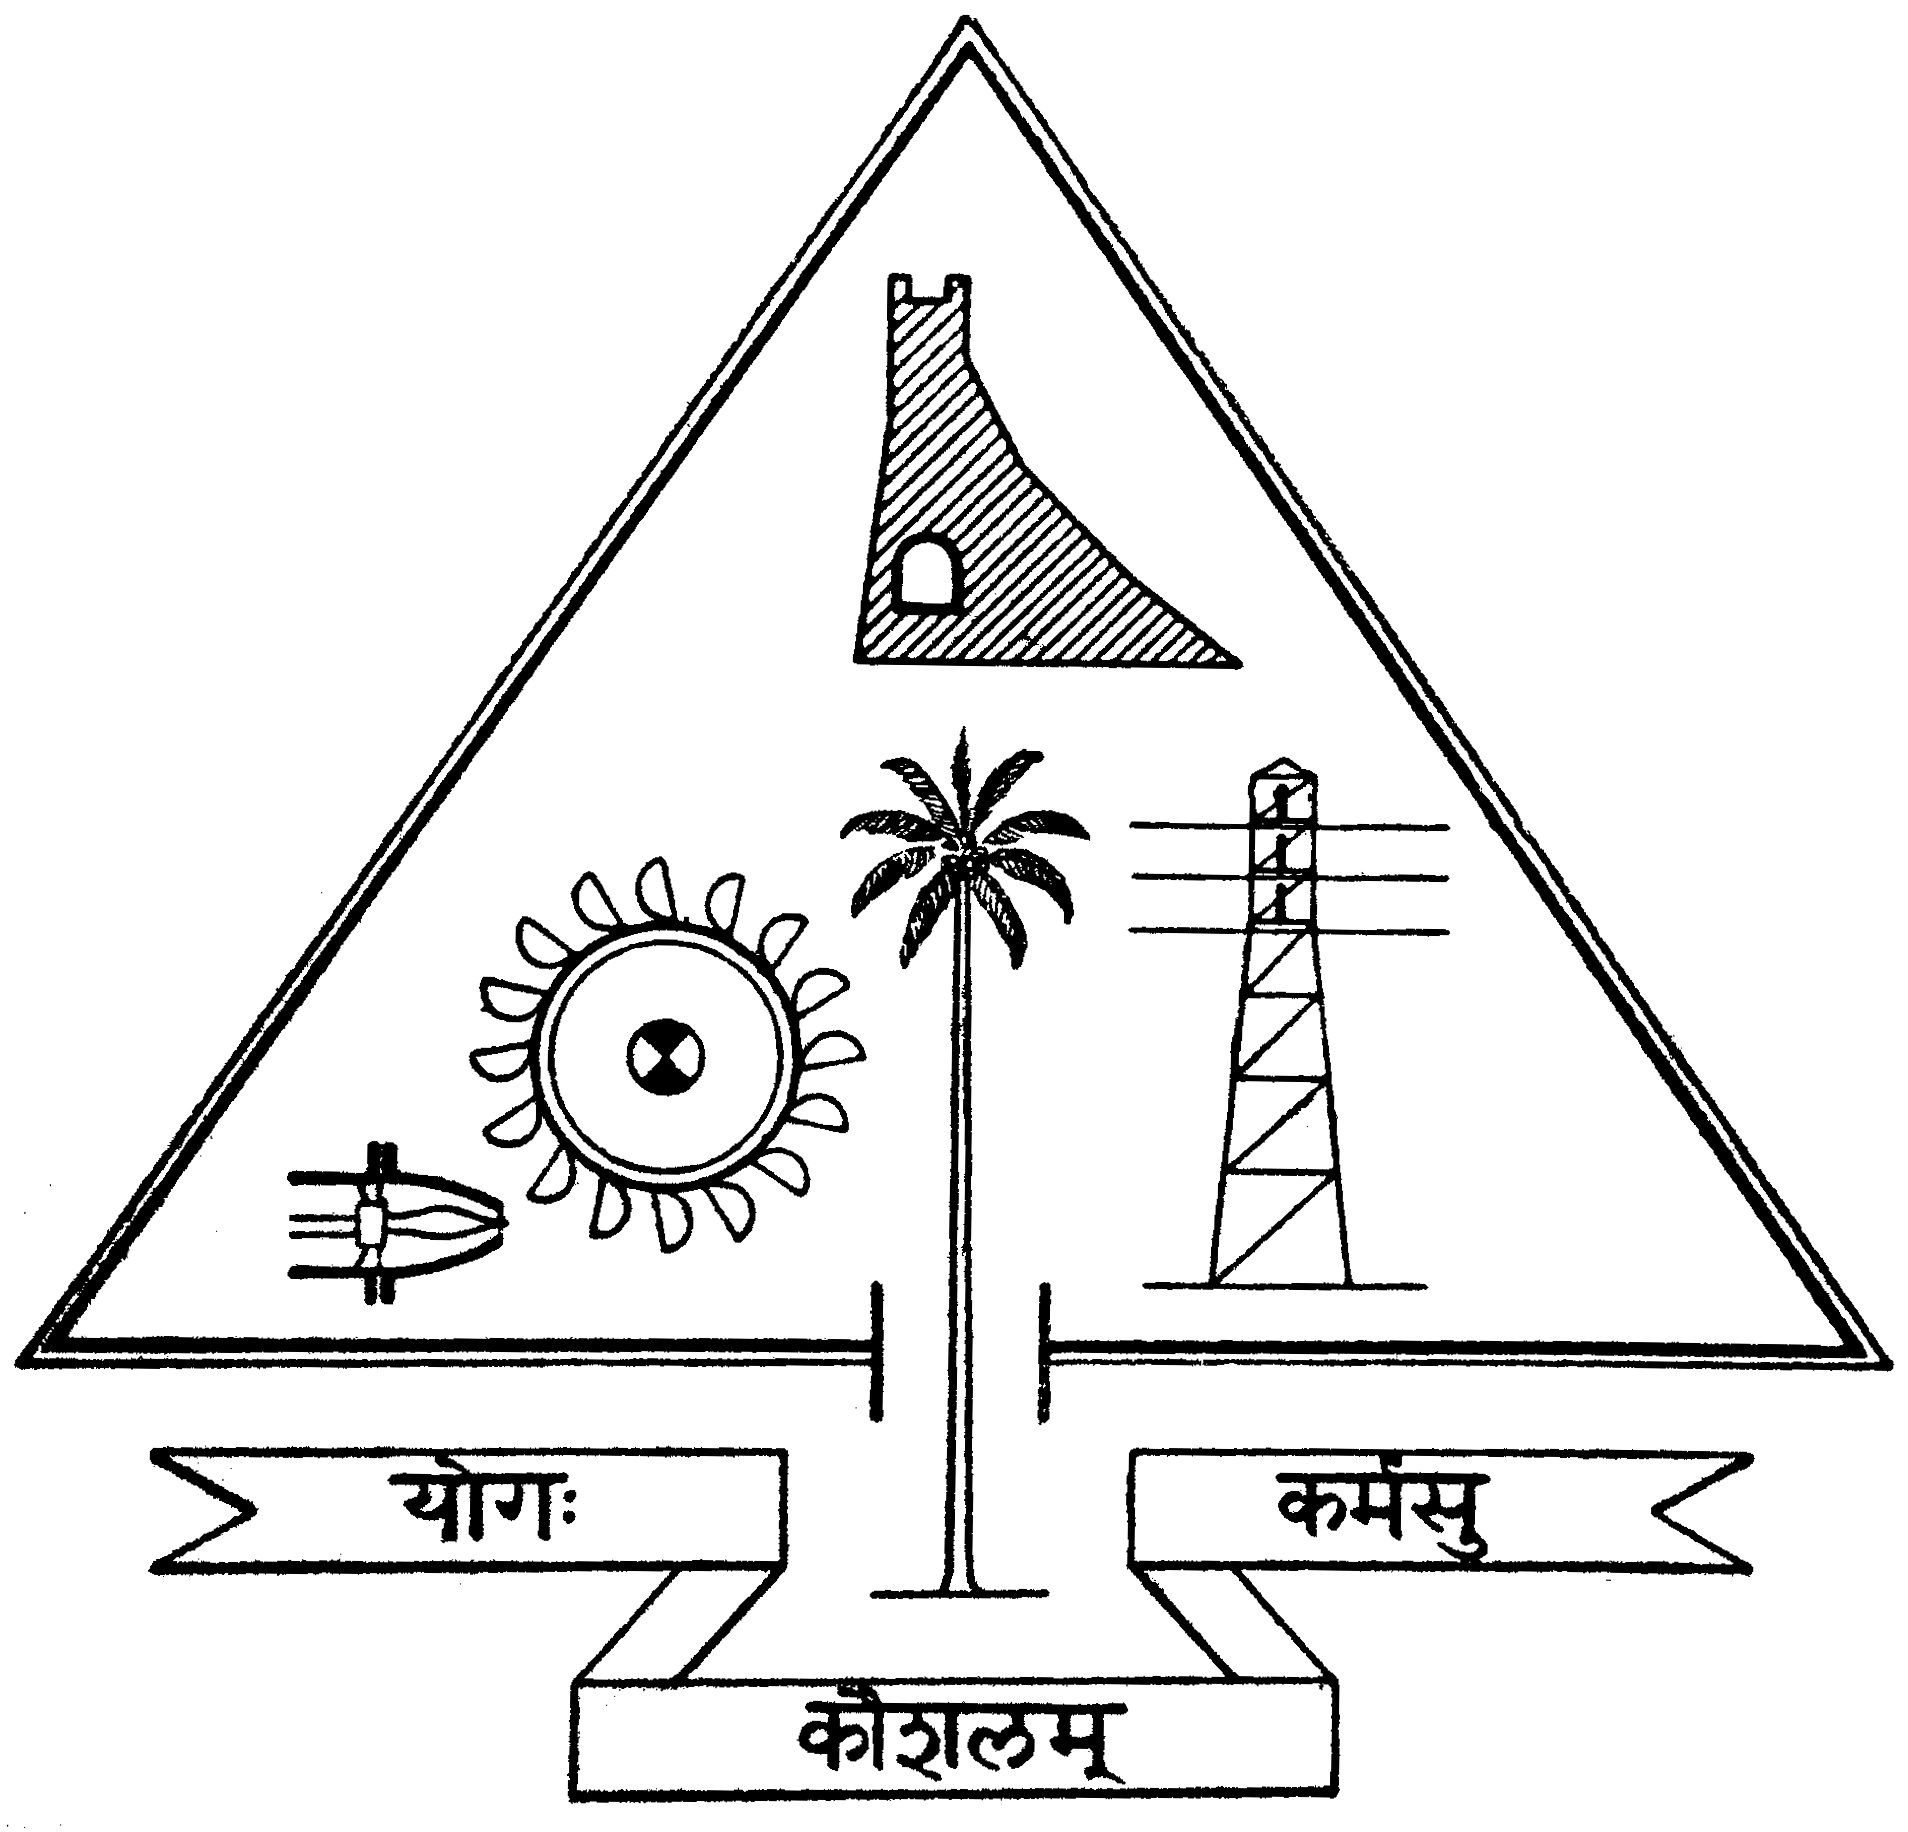
\includegraphics[height=1.4in, width=1.4in]{figures/gectemblem}\\
	Department of Electrical Engineering \\
	Government Engineering College  \\
	Thrissur-680009, Kerala, India \\
}
\date{OCTOBER - 2018}
\maketitle

\section*{DECLARATION\centering}
   	I undersigned hereby declare that the Seminar report ``Impedance-Based Battery Management System For Safety Monitoring Of Lithium-Ion Battery", submitted for partial fulfillment of the requirements for the award of degree of Bachelor of Technology of the APJ Abdul Kalam Technological University, Kerala is a bonafide work done by me under supervision of Prof. Uma Syamkumar and Dr. Ramesh Kumar P. This submission represents my ideas in my own words and where ideas or words of others have been included, I have adequately and accurately cited and referenced the original sources. I also declare that I have adhered to ethics of academic honesty and integrity and have not misrepresented or fabricated any data or idea or fact or source in my submission. I understand that any violation of the above will be a cause for disciplinary action by the institute and/or the University and can also evoke penal action from the sources which have thus not been properly cited or from whom proper permission has not been obtained. This report has not been previously formed the basis for the award of any degree, diploma or similar title of any other University. \\
\vspace{0.3in}
\newline
	\begin{tabular}{lp{3.5in}r}
		Thrissur  & & \\
		Date : 10/10/2018 & & \textbf{Alin Anto}
	\end{tabular}
\thispagestyle{empty}
\clearpage

\section*{ACKNOWLEDGEMENT\centering}
	I wish to place on record my hearty thanks and sincere gratitude to my supervisor Prof. Uma Syamkumar and Dr. Ramesh Kumar P  for their invaluable guidance, suggestions and constant encouragement. \\
\vspace{0.3in}
\newline
	\begin{tabular}{lp{3.5in}r}
		Thrissur  & & \\
		Date : 10/10/2018 & & \textbf{Alin Anto}
	\end{tabular}
\thispagestyle{empty}
\clearpage

\begin{abstract}
Multi-frequency impedance measurements have been recognized as a technique for the
monitoring of individual calls in Lithium-ion (Li-ion) batteries. However, its practical
introduction for battery management has been slow, mainly due to added size and larger
operating power requirements. Here, we describe a small, low-power, multi-frequency (1-1000
Hz) impedance-based battery management system (BMS) for multi-cell batteries of varying
capacities. This BMS ensures battery safety and efficiency by tracking and acting on emerging
mismatches and other electrical and thermal abnormalities in each individual cell without adding
cost, volume, weight and power, compared to conventional BMSs. Multi-cell batteries face a
unique problem that single cell Li-ion batteries do not: mismatching of one or more cells is
detrimental to the safety and efficiency of the entire battery. Thus, cell matching is an important
first step required for safe operation of multi-cell Li-ion batteries. Cell mismatch can occur due
to battery over-discharge, overcharge, internal and external shorts, etc., or even when leaving a
battery unused for an extended period (calendar aging). Predicting a mismatch is essential for a
battery’s thermal safety and electrical efficiency. Conventional BMSs typically monitor cell
voltages and surface temperature. However, these measurements and related protocols have not
succeeded in ensuring battery safety or improving efficiency. Data for batteries with intentionally
calendar-aged and over-discharged cells convincingly demonstrate that such BMSs cannot
identify cell mismatches and emerging failures. In contrast, the impedance-based BMS,
described here, tracks, identifies, and acts on changes in the internal state of each cell
continuously in real time, including battery charging, discharging, and at rest.
\end{abstract}

	\pagenumbering{roman}
	\tableofcontents
\clearpage 
	\addcontentsline{toc}{chapter}{List of Figures}
	\listoffigures
\clearpage
	\addcontentsline{toc}{chapter}{Nomenclature} 
	\chapter*{Nomenclature}

\textbf{List of symbols} \vspace{0.3in} \\
\begin{tabular}{ll}
$E_{cv}$ & Cell voltage  \\
$R_s$ & Electrolyte resistance \\
$T_{int}$ & Cell Internal temperature  \\
$T_{surf}$ & Cell surface temperature  \\
$[Li+]$ & Concentration of Lithium anion \\
\end{tabular}\\

\vspace{1.5in}

\textbf{Acronyms} \vspace{0.3in} \\
\begin{tabular}{ll}
BMS & Battery Management System\\
USA & United States of America \\
Ah & Ampere-Hour \\
SoC & State Of Charge\\
SOH & State Of Health\\
FOD& Foreign Object-Debris\\
SEI& Solid-Electrolyte-Interphase\\
BITS & Battery Internal Temperature Sensor\\
ADC& Analog-to-Digital Converter\\
USB & Universal Serial Bus\\
Li & Lithium\\
Li+ & Lithium anion
\end{tabular}

\clearpage
	\pagenumbering{arabic}
	\chapter{Introduction}

\hspace{0.5cm} 
Matching of cells in a battery is the number one priority for best battery performance. Yet, little attention is paid to ensure that all cells remain matched throughout the battery lifecycle. Normal operations as well as calendar aging cause the battery to mismatch. Permanent or intermittent external short of even a single cell in a multicell battery also causes cell mismatch. In order to ensure safety, a battery management system (BMS) should identify mismatched cells throughout the battery lifecycle. In most cases, cells are rarely monitored for cell matching. Typically, equipment that uses Li-ion batteries has a BMS that only monitors cell voltage $E_{cv}$ and cell surface temperature $T_{surf}$\cite{dey2016sensor}. Some BMS also monitor ampere-hour capacity (Ah-capacity)\cite{giegerich2016open}, and much less often internal impedance $R_s$ at a single frequency \cite{taylor2012system} -\cite{waag2014critical}, typically 1 kHz. In order to fully characterize the impedance, the BMS should be able to accurately measure in-phase and quadrature (i.e., real and imaginary) components over three decades, typically between 1 and 1000 Hz. By monitoring both amplitude and phase shift at multiple frequencies, the BMS will fully characterize the impedance of the anode, cathode, and the electrolyte. To prevent interfering with the equipment that the battery is powering, such a BMS should not add more than a few mV ac voltage between the cell terminals. A BMS with a singlefrequency- impedance-meter, the only type described so far, essentially only monitors $E_{cv}$, $T_{surf}$ , and the electrolyte resistance, $R_s$. A BMS that monitors only the maximum and minimum $E_{cv}$, single frequency impedance, battery’s Ah-capacity, and $T_{surf}$ of a few cells, may not identify mismatched cells. Test data presented below show that monitoring only $E_{cv}$ and $T_{surf}$ does not ensure adequate electrical and thermal safety. In this paper, we demonstrate that multifrequency impedance data (real and quadrature covering three decades of frequency domain) can be correlated reliably to evolving cell mismatches under three common scenarios: cycle life aging, calendar life aging, and overdischarge and overcharge. We also describe a new and practical BMS that in addition to the conventional $E_{cv}$ monitor contains a multifrequency impedance meter. Our impedance-based BMS has small size (10 × 10 cm), low power demand (6 V; 0.75 A dc), and standalone operation (no need for an external processor to manage the battery and direct commands to external controls such as switches and relays).

\section{Test setup}

\hspace{0.5cm} 
Five different types of Li-ion batteries are used in the tests. For all batteries, new cells, rated to 5.3 Ah capacity,  are selected (Swing 5300 model, Boston Power, Boston, MA, USA). The new cells were cycled twice between 2.7 and 4.2 V at $C/4$-rate, brought to 50\% state of charge ($SoC$), rested overnight at room temperature before screening for matching and making the batteries. Only cells that matched within 3 mV, and in multi-frequency impedance within $\pm$0.5\%, and identical in Ah capacity were selected for assembling batteries. Within one day after the cell screening and selection, one three cell battery, one six-cell battery and two individual cells for abuse (over-discharge and overcharge) tests were reserved. Tests on the three-cell battery started within one day after assembly. The six-cell battery and the two spare cells were stored under ambient conditions for six months before testing. The cells were fully ventilated from all sides to prevent unbalanced thermal constrains. The cells were separated by 5 mm air gap from each other. The battery was raised 5 mm above the resting table, and its top was fully open to air to minimize cell-to-cell heat transfer. 

\subsection{Definitions of normal, bad, and matched cells}

\hspace{0.5cm} 
A new cell is normal if 1) its Ah-capacity determined at $C/4$ rate discharge–charge cycle is the same or better than the nameplate capacity and 2) its internal real and quadrature impedances at 1 kHz, 10 Hz, and 1 Hz all match within $\pm$0.5\% of multiple cells from the same lot. An aged cell is normal if 1) its Ah-capacity determined at C/4 rate discharge–charge cycle follows a linear decay that does not exceed 20\% of its nameplate capacity at the manufacturer-specified end of life and 2) its internal real and quadrature impedances at 1 kHz, 10 Hz, and 1 Hz all match within $\pm$5\% of the new normal cell. A cell is bad, within the context of this work, if it has been over-discharged ($E_{cv}$ dropping almost to zero volt) or overcharged ($E_{cv}$ reaching few hundred milli-volts above 4.2 V) at least once. Cells are matched if their voltages are within $\pm$5 mV at full charge, Ah-capacities are within $\pm$5 mAh, and their impedances have a $\pm$0.5\% at each of the following frequencies: 1 kHz, 100 Hz, 10 Hz, and 1 Hz. 



	\chapter{Cell Monitoring}

\hspace{0.5cm} 
Using new, cycle-aged, calendar-aged, or over-discharged cells, the shortcomings of cell voltage, surface temperature, and electrolyte resistance monitors to detect and predict cell mismatch is verified experimentally. These results highlight that bad and normal cells are nearly identical in their $E_{cv}$ and $T_{surf}$ values, while high-frequency impedance is concurrently influenced by electrolyte temperature, cell aging and changes in Li+ concentration. 

\section{Cell Voltage Monitor}

\hspace{0.5cm}
$E_{cv}$ monitoring is a commonly incorporated feature in conventional BMS. Its main role in a BMS is to ensure that no cell in the battery exceeds preset upper and lower limits, respectively. During current flow (when charging or discharging), $E_{cv}$ is dominated by three different polarization effects: 1) activation and diffusion at the anode and the cathode, 2) resistive drop across the electrolyte, with relatively insignificant contributions from 3) foreign-object-debris ($FOD$). FOD refers to any nonfunctional material that despite careful cell manufacturing may find its way into the cell. For example, FOD include copper and aluminum particulates from current collectors. FOD can cause internal short circuit, chemical changes induced by over-discharge, and chemical and physical changes after cycle and calendar aging. As a result, $E_{cv}$ of cells with FOD, over-discharge and age abnormalities will be quite similar to those of cells without those abnormalities. FOD, over-discharge, and aging are the main reasons why cells become mismatched; however, cell voltage monitoring alone cannot identify cell mismatch.

\vspace{0.5cm}
The data in Figure \ref{emf1} demonstrate that in a six-cell battery with five aged cells and one over-discharged cell, the $E_{cv}$ of all six cells remained close (standard deviation under $\pm$5 mV), down to 30\% SoC during discharge, and at all SoC during charge. Only below 20\% SoC did the cell voltages start to deviate markedly from each other, with the over-discharged (bad) cell deviating most at full discharge. At full discharge, the bad cell was at 2.387 V, i.e., 313 mV below the manufacturer-recommended 2.7 V limit for the cell, while the voltage of the entire battery reached only its lower limit (16.2V), falsely suggesting that each cell was at the 2.7 V limit ($2.7V\ast6=16.2V$). A cell-voltage monitor in a BMS is thus not always capable of identifying mismatched and over-discharged cells, and will miss bad cells discharging far below their recommended limit, which might cause a battery fire.

\begin{figure}
	\includegraphics[width=11cm,height=8cm]{figures/emf_monitor.png}
	\centering
	\caption{
		Cell voltages(discharge and charge of a six cell Li-ion battery containing five matched and one over-discharged cell.)}\label{emf1}
\end{figure}

\section{Surface Temperature Monitor}

\hspace{0.5cm}
Next monitor method is cell surface temperature $T_{surf}$ in order to identify cell mismatching. Battery voltage (indicating the discharge{/}charge cycle) and surface temperature variations for one normal and the bad (previously over-discharged) cell in the six cell battery from Figure \ref{emf1} are plotted in Figure \ref{tem1} The surface temperatures of the normal and over discharged cells were virtually identical until the battery was fully drained (at 687 min time point). For a completely drained battery, the surface temperature of the bad cell deviates by no more than one degree from normal cell temperature ($24^oC$). In other words, surface-mounted temperature sensors can barely discriminate an over-discharged (i.e., mismatched) cell from normal cells. Similarly, for batteries with new and cycle-aged cells, individual cell $T_{surf}$ values were identical to each other. In addition to not being adequate in discriminating bad cells from normal ones, surface-mounted sensors have several more shortcomings. $T_{surf}$ sensors are slow in responding to changes in the discharge currents flowing through the cell and they cannot identify when the cell is being overcharged. Furthermore, when a battery is rapidly charged or discharged, $T_{surf}$ values do not indicate impeding damage to the interior of the cell. For example, through the discharge–charge cycle at $1^oC$ rate of a three-cell battery, $T_{surf}$ remained well within $20^oC$ to $40^oC$ (see Figure \ref{tem2}). This temperature range is considered “safe” by most battery safety standards. However, the cell’s internal temperature exceeded $60^oC$, less than $20^o$ below $80^oC$, considered unsafe by most standards.

\begin{figure}[H]
	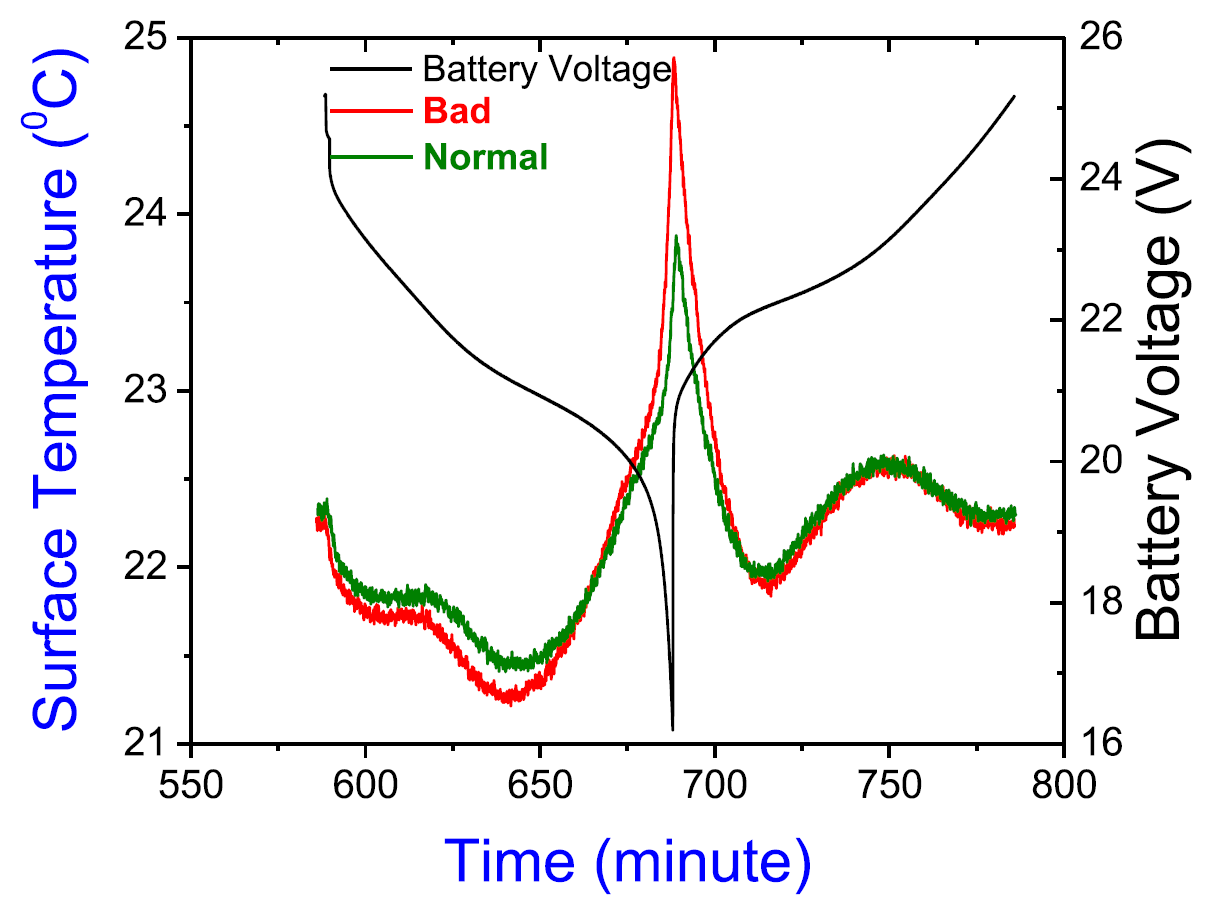
\includegraphics[width=11cm,height=8cm]{figures/tem1}
	\centering
	\caption{Surface temperatures of one aged (normal, green) and one over-discharged (bad, red) cell.}\label{tem1}\vspace{0.5cm}

	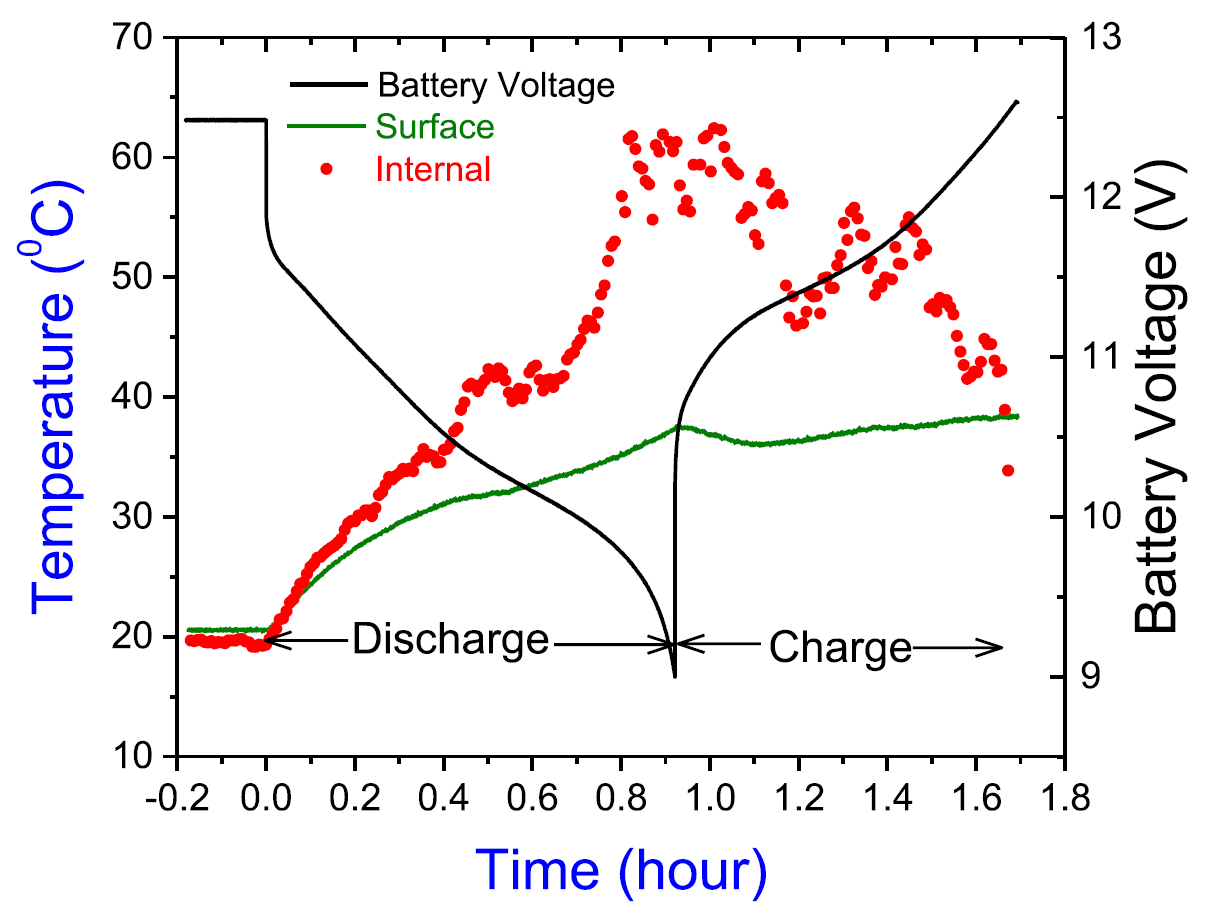
\includegraphics[width=11cm,height=8cm]{figures/tem2}
	\centering
	\caption{
		Surface temperature (green) and internal (anode) temperature (red) of one of the cells in a cycle-aged three-cell battery.}\label{tem2}
\end{figure}

\section{Electrolyte Resistance Monitor}

\begin{figure}[H]
	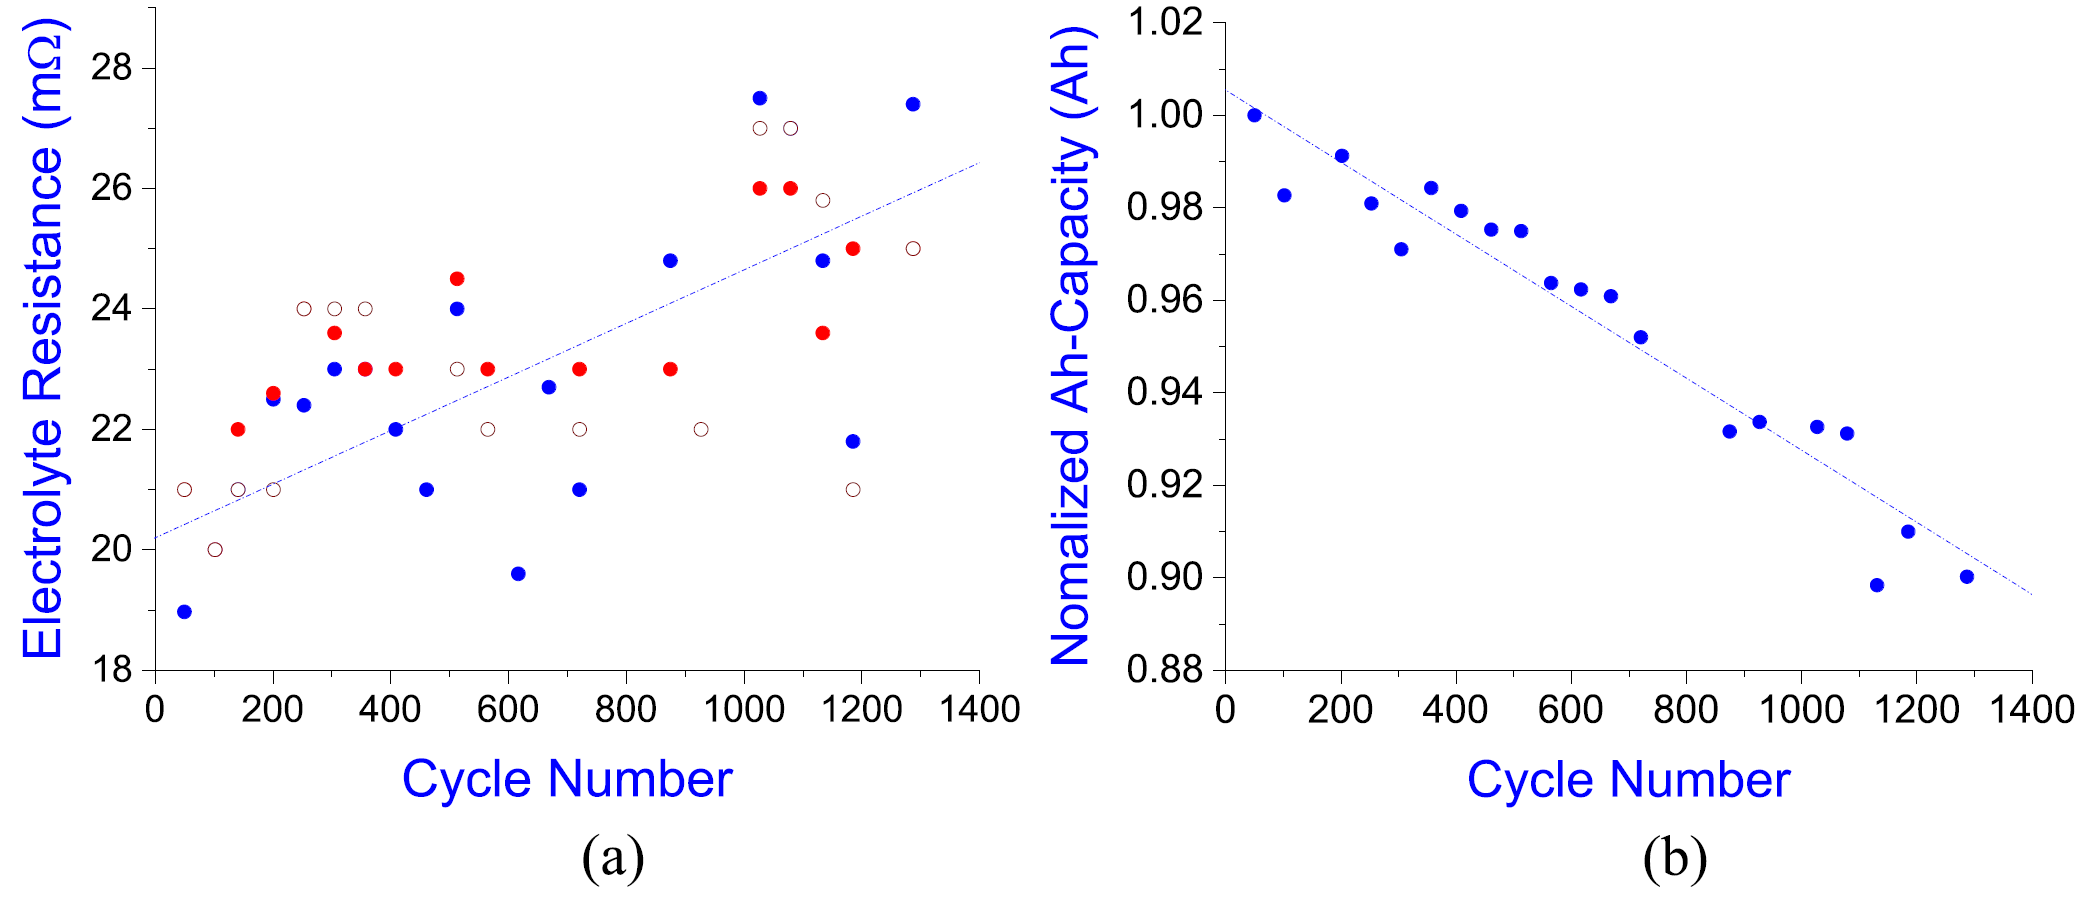
\includegraphics[width=16cm,height=7cm]{figures/electrolyte1}
	\centering
	\caption{(a) Effect of cycle life on electrolyte resistance, $R_s$ , in three identical Li-ion cells. (b) Ah-capacity as a function of cycle life for one of the three cells.} \label{electrolyte1}
\end{figure}

\hspace{0.5cm}
$R_s$  reportedly serves two purposes: 1) to identify a cell’s internal temperature; 2) to estimate cell aging and health. In both cases, $R_s$ is determined from measured cell impedance at a single frequency. While single-frequency impedance monitoring can estimate cell cycle-life aging, it is valid only if impedance is measured after the cell is rested for extended time at constant ambient temperature (see Figure \ref{electrolyte1}). Furthermore, $R_s$ can be correlated to the temperature of the electrolyte only if age-induced changes in electrolyte resistance are ignored and no current is flowing through the cell. For example, Li+ cations, released into the electrolyte from the anode during discharge, are taken into the cathode; the opposite process occurs during charge. However, the rates of release and intake, reflecting the anode and cathode reaction kinetics, respectively, differ (the release rate is higher than the intake). The rate differences between the two electrodes result in $[Li+]$ buildup in the electrolyte. $[Li+]$ change during discharge and charge results in a change in electrolyte resistance.

\vspace{0.5cm}
In the example shown [see Figure \ref{electrolyte2} (a)], during cell charge and discharge at $C/2$-rate, $R_s$ varied between 22.7 and 25 $m\Omega$. This 14\% variation between $R_s$ maximum and minimum is comparable to the 30\% change observed due to cycle life aging [see Figure \ref{electrolyte1} (a)]. Therefore, monitoring cell aging from high-frequency impedance data may be feasible only if impedance is measured when the cell is at rest, and care is taken to maintain the cell at the same internal temperature between each measurement [see Figure \ref{electrolyte1} (a)]. The variation in $R_s$ can be caused by changes in electrolyte temperature as well as changes in $[Li+]$ in the electrolyte. If impedance measurements are used in estimating electrolyte temperature during charge and discharge, the current-induced changes in $[Li+]$ will introduce errors in those estimates, as demonstrated in the discrepancy between the cell internal temperature (estimated from high-frequency impedance) and the surface temperature [see Figure \ref{electrolyte2} (b)]. Compared to $T_{surf}$ , the internal temperature behaved differently after an initial rise to $28^oC$ during discharge, it subsequently dropped. The drop in internal temperature is an artifact, best explained by the differences in reaction kinetics between the anode and the cathode and $[Li+]$ changes during discharge.

\begin{figure}[H]
	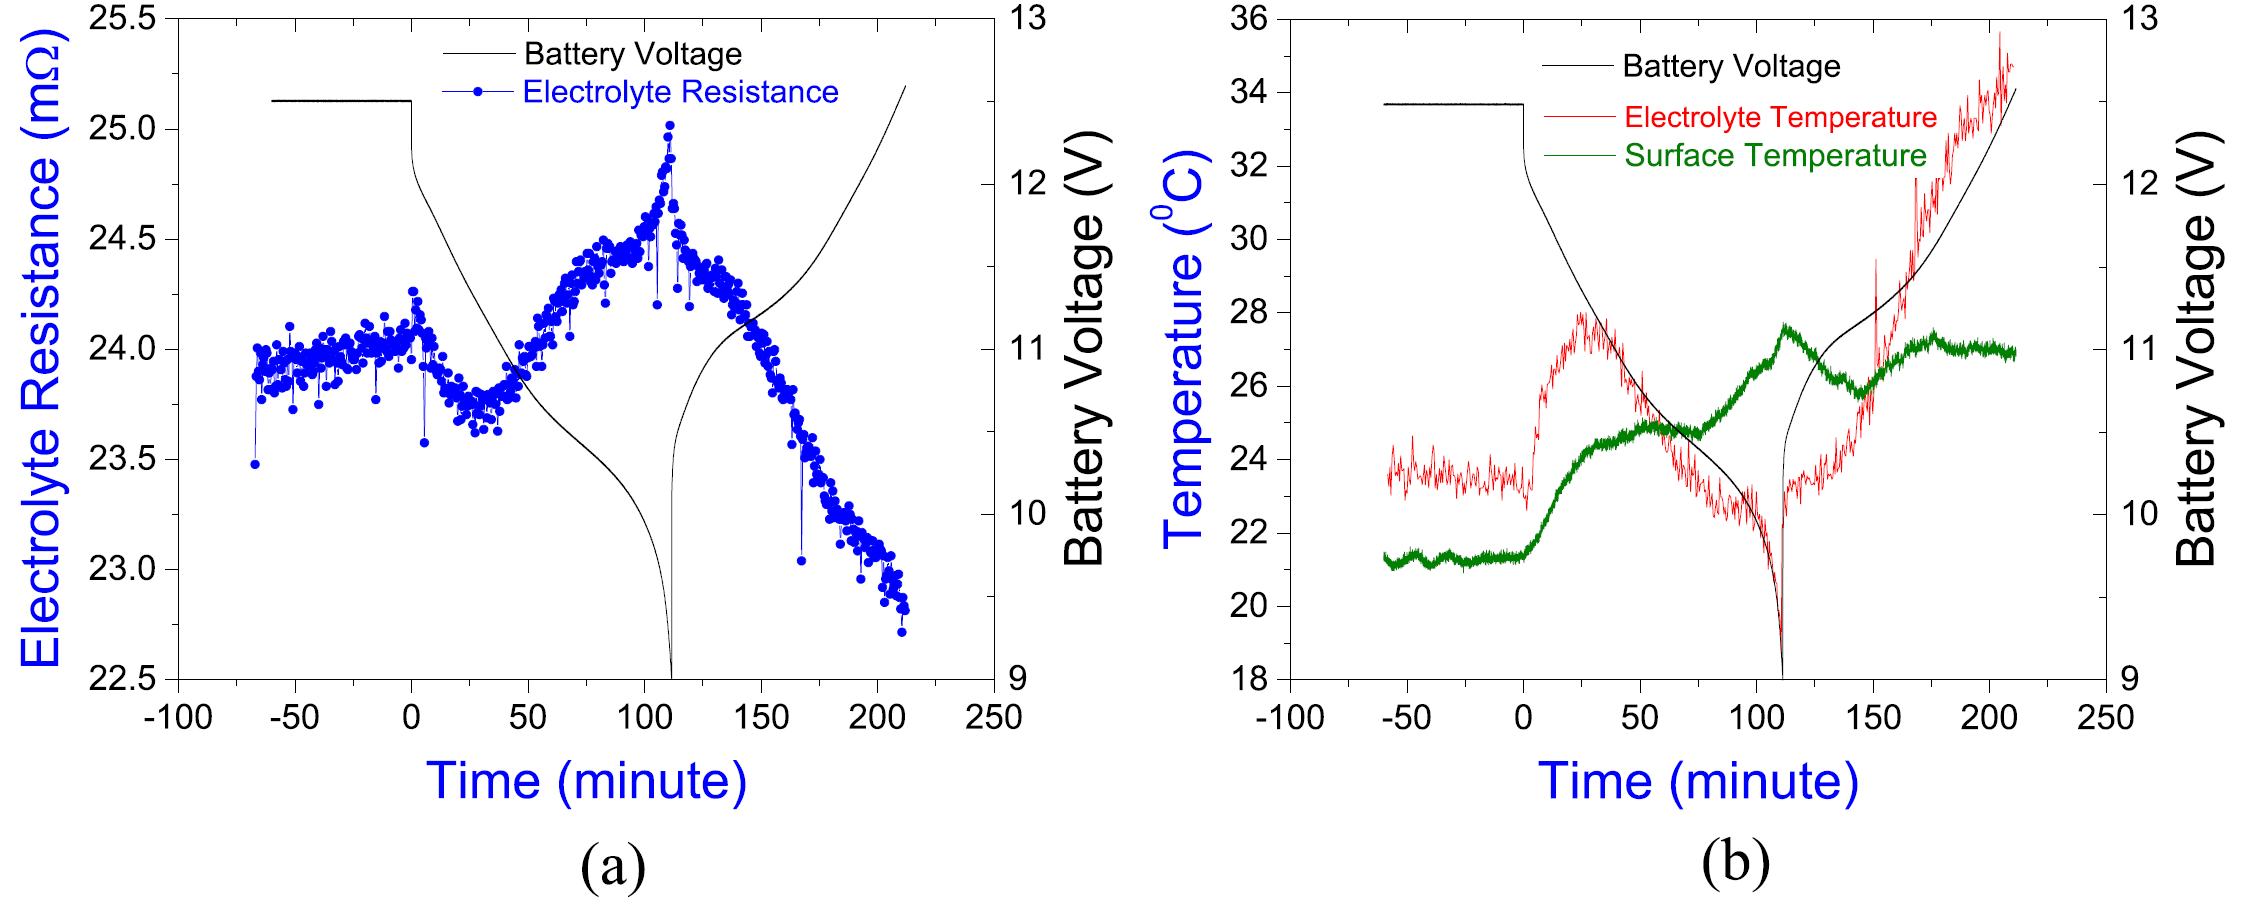
\includegraphics[width=16cm,height=6cm]{figures/electrolyte2}
	\centering
	\caption{
		(a) Electrolyte resistance, Rs of one cell during a single cycle of discharge{/}charge of a new and matched three-cell battery (b) Internal temperature (red) of the same cell and surface temperature (green).} \label{electrolyte2}
\end{figure}

\section{Impedence approach to identify Cell miss-match}

\begin{figure}[H]
	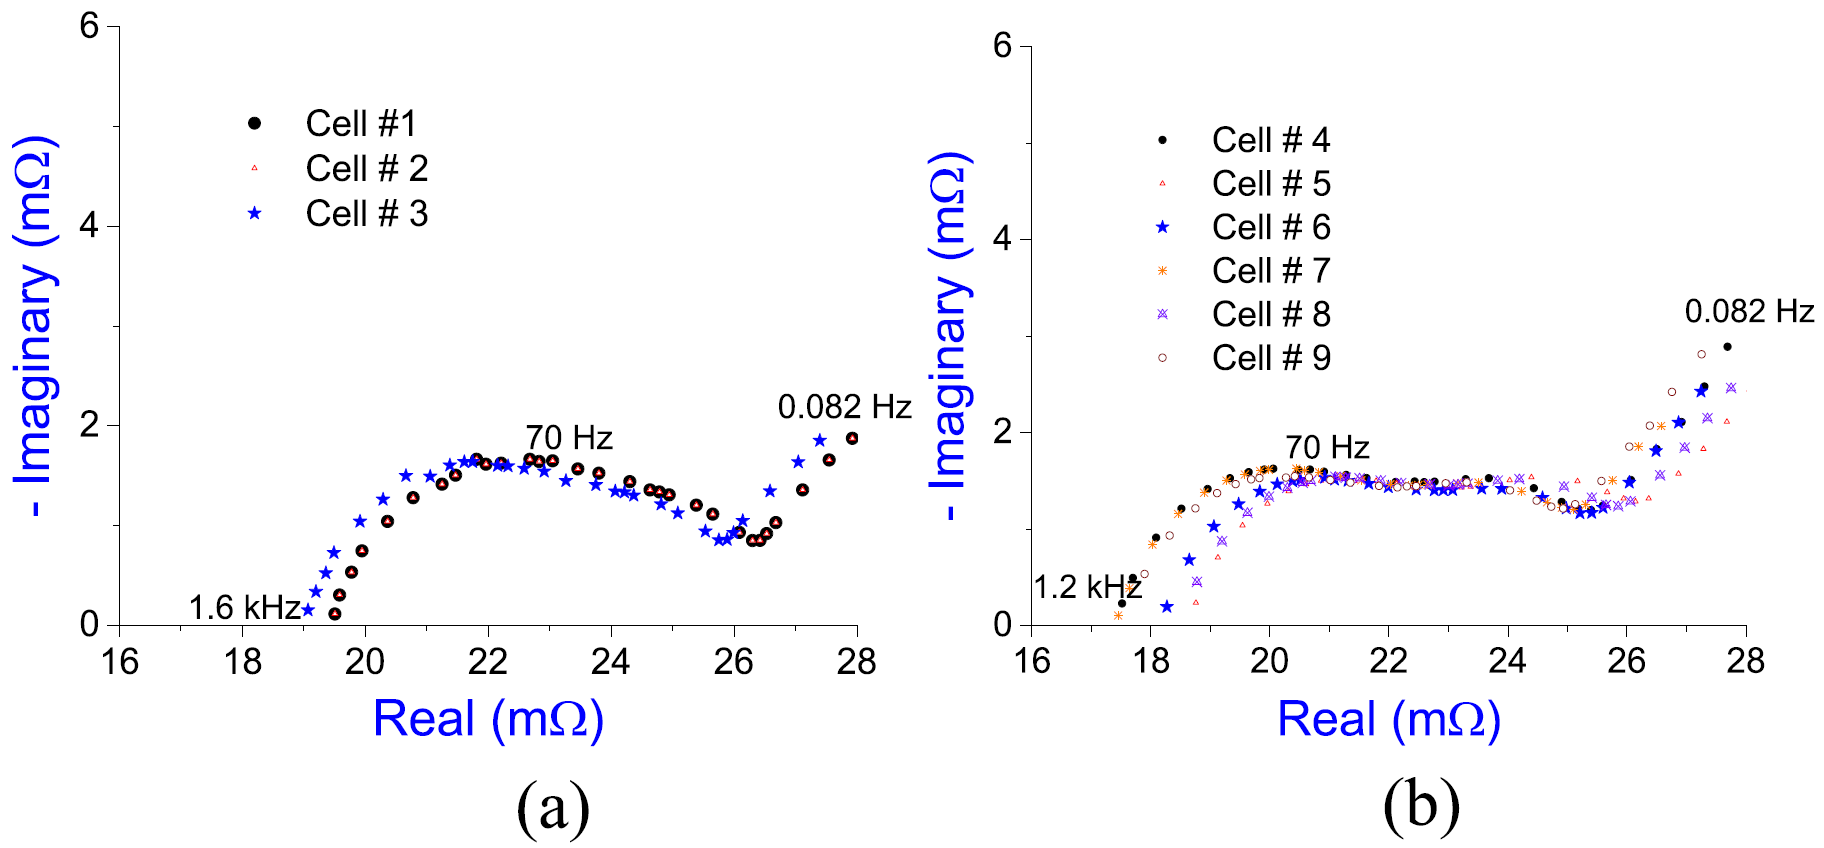
\includegraphics[width=16cm,height=7cm]{figures/impedence1}
	\centering
	\caption{Impedance behavior of cells in different Li-ion batteries containing: (a) three new, matched cells; (b) six matched, calendar-aged cells.} \label{impedence1}
\end{figure}

\hspace{0.5cm}
A Li-ion cell is a multi-component system, consisting of an anode, cathode, electrolyte, separator, and current collectors. The solid-electrolyte-interphase (SEI) layer is most sensitive to temperature and least sensitive to SoC. Current flow changes SEI layer’s temperature, therefore measuring the impedance allows to monitor the cell’s anode and cathode temperatures. Low-frequency impedance is influenced by both SoC and internal temperature. However, separating their effects can be challenging. $R_s$ , best identified as high-frequency impedance, is also sensitive to temperature, $[Li+]$ and cell aging. Thus, a multi-frequency impedance meter equipped to measure both phase shift and amplitude is required to discern changes occurring in the anode, cathode, and the electrolyte.

\begin{figure}[H]	
	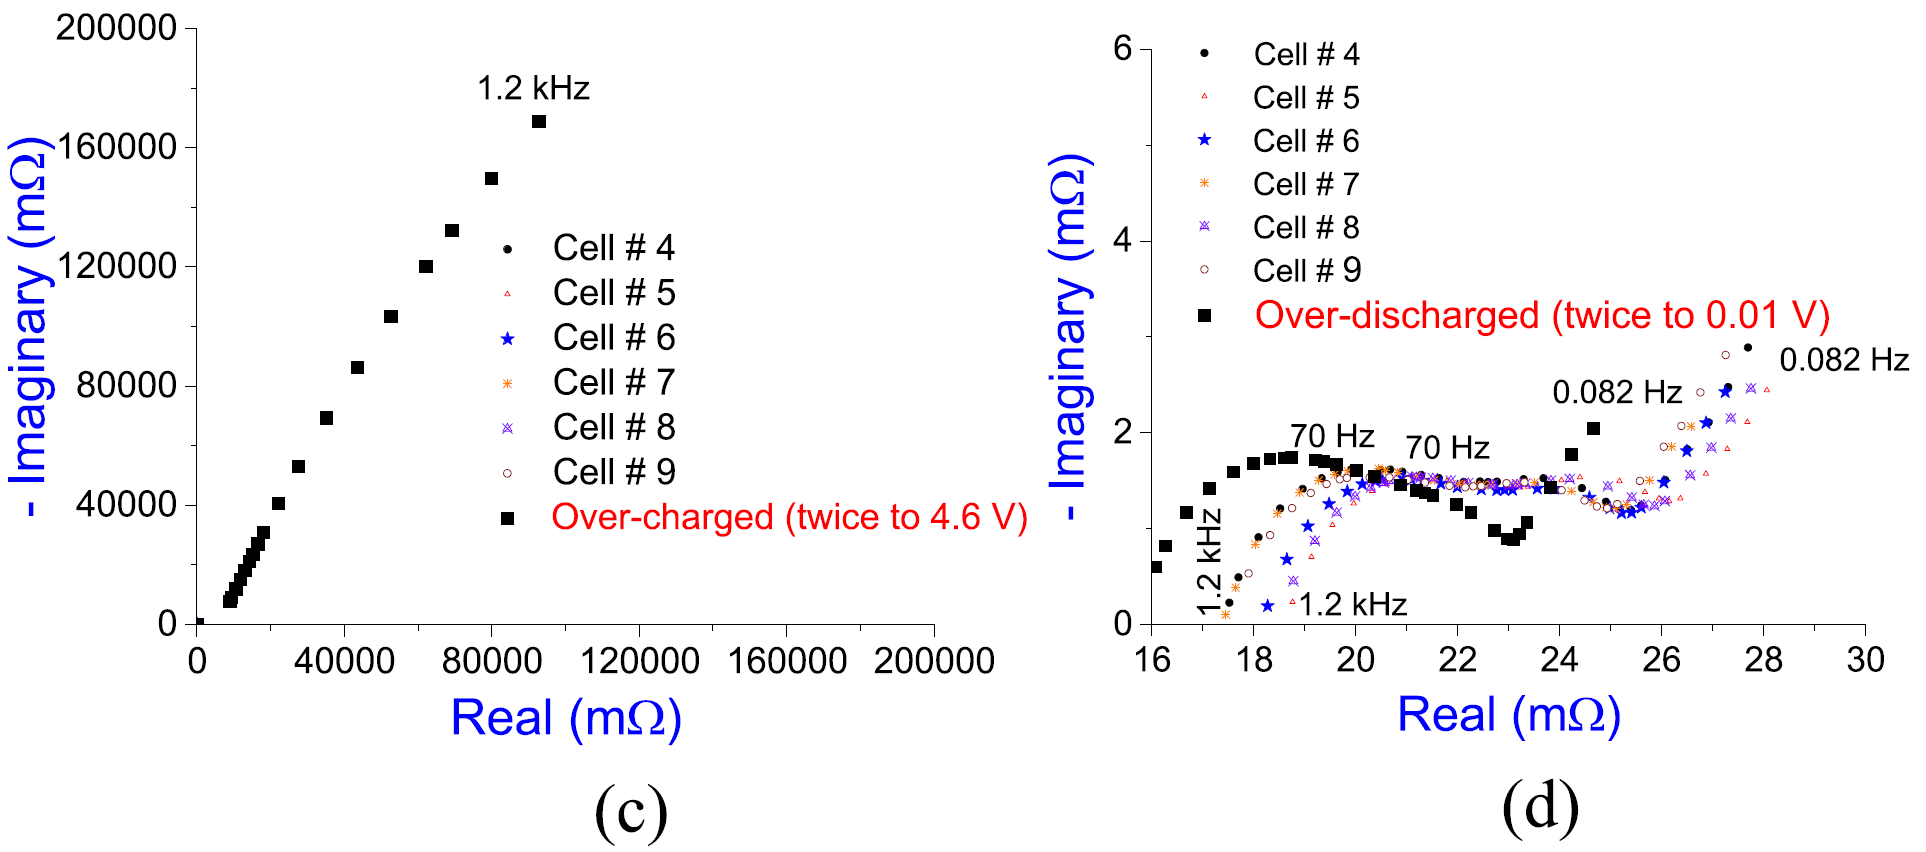
\includegraphics[width=16cm,height=7cm]{figures/impedence2}
	\centering
	\caption{Impedance behavior of cells in different Li-ion batteries containing: (a) five matched, calendar-aged cells and one overdischarged cell; (b) five matched, calendar-aged cells and one overcharged cell.} \label{impedence2}
\end{figure}

Figure \ref{impedence1} (a) shows impedance data for three cells in a three-cell battery matched within $\pm$0.5\%. Figure \ref{impedence1} (b) shows impedance data for each of the six cells in a six-cell battery after aging. Individual cell’s impedance drifted from its original value by more than 6\% [see Figure \ref{impedence1} (b)], while the spread in impedance values after aging also increased. Also examined are two modified six-cell batteries that had five cells aged as the ones in Figure \ref{impedence1} (b), with the sixth cell replaced by an over-discharged cell, or by an overcharged cell, respectively. The purpose of deliberately over-discharging one cell in the six-cell battery is to demonstrate: 1) cell voltage monitors are unable to identify an over-discharged cell in the battery; and 2) impedance technique can identify the over-discharged cell event, before the event causes internal short. The impedance of the over-discharged cell after resting the cell overnight at 50\% SoC compared to the impedance of the five normal aged cells is markedly different [see Figure \ref{impedence2} (a)].  Figure \ref{impedence2} (b) shows impedance data for all six cells in the battery with one cell overcharged twice by charging up to 4.6 V (4.2 V is the upper limit for normal charge). The impedance of the over-discharged cell is 100000 times larger than the rest of the cells.







	\chapter{Impedance-Based BMS}

\hspace{0.5cm}
Commercial impedance meters have a wide range of capabilities, but they are rarely used as BMS. Besides size, weight, and power-consumption, they are not designed to monitor simultaneously multiple cells in a battery. Furthermore, conventional BMS that monitor impedance measure only its amplitude at a single frequency, typically at 1 kHz, and are therefore not suitable for properly characterizing a cell mismatch. The data in Figure \ref{impedence1} and Figure \ref{impedence2} demonstrate that cell impedance is indicative of calendar aging, over-discharging, and overcharging. Characterizing the impedance of a cell requires amplitude and phase measurements at multiple frequencies. Impedance based BMS is designed for such measurements. Figure \ref{BLOCK} shows such a impedance-based BMS, Battery Internal Temperature Sensor-based BMS, or BITS-BMS. It is designed to monitor each of up to 16 cells in a multi-cell battery that generates up to 80 V and 50 Ah, with no limit on the battery discharge–charge rates. This $10\ast10$ cm unit, powered by a 6 V, 0.75A dc power supply, is a standalone unit, i.e., requires no computer control to operate. It is ON when the power supply is ON, when it starts collecting data for each cell through a 16-cell multiplexer. 

\begin{figure}[H]
	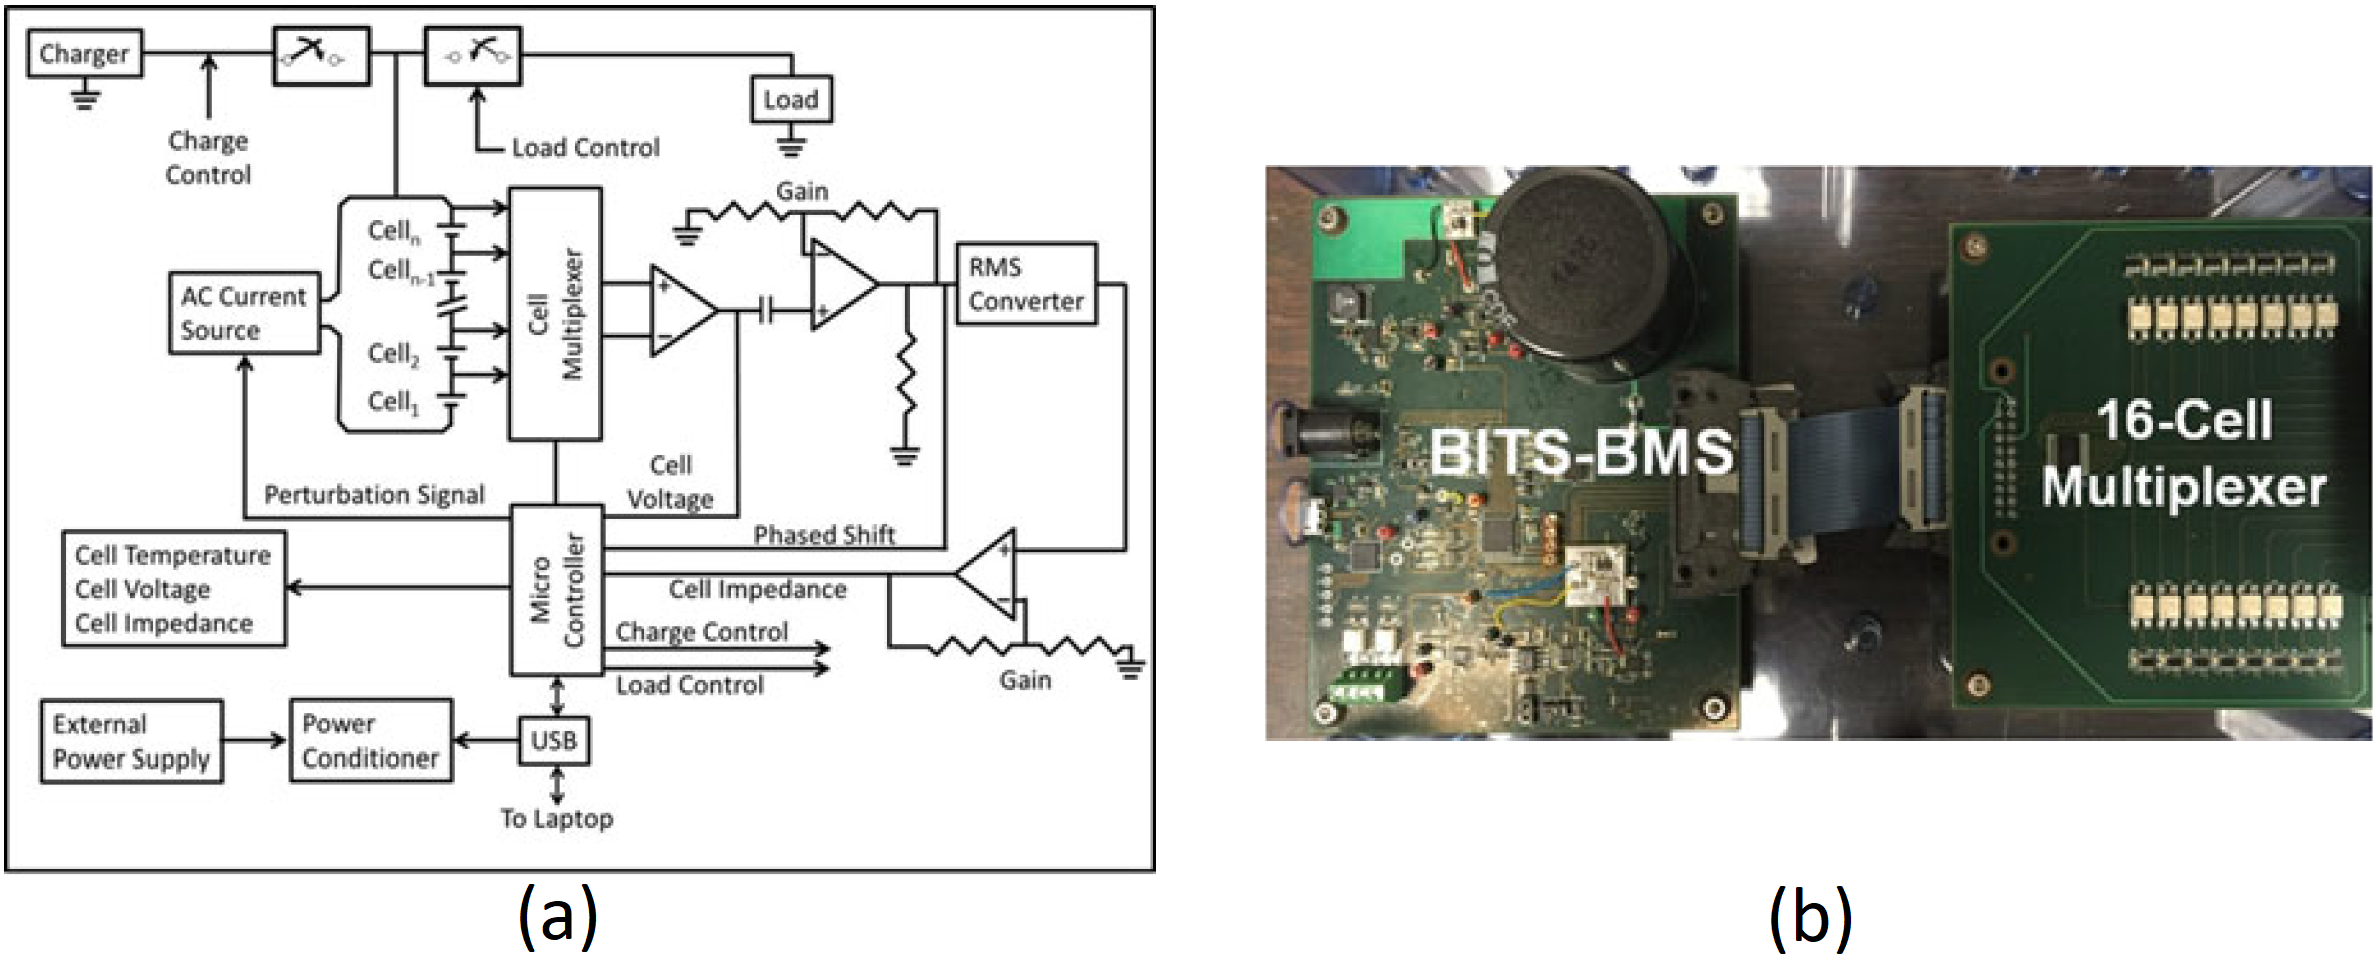
\includegraphics[width=16cm,height=6cm]{figures/BLOCK}
	\centering
	\caption{(a) Impedance-based BMS: schematic describing the main components; (b) photo of the fully operational prototype and a 16-cell multiplexer.} \label{BLOCK}
\end{figure}

\section{BITS-BMS Principle of Operation}

\hspace{0.5cm}
The BITS-BMS collects impedance data by injecting a small amplitude ac current signal of fixed amplitude (typically 100mA rms for a 50 Ah cell; or 25 mA rms for a 5 Ah cell) at multiple frequencies in the 1 Hz to 1 kHz range. This ac signal is generated via a programmable microcontroller outputting sinusoidal waveforms of fixed frequencies and fixed amplitude through a current pump. The ac current from the pump is directed toward the cells through the multiplexer, one cell at a time. The ac current perturbs the cell eliciting a voltage response. The BMS generates the perturbation signal through a constant-current source, thus ensuring identical amplitude current passes through each cell in the battery. At each frequency, the circuits following the multiplexer measure the amplitude of the resulting voltage and phase shift between the current and the voltage. The voltage amplitude is a direct measure of the cell impedance, and the phase shift is correlated to the anode temperature and cathode temperature.

\vspace{0.5cm}
The BMS has no restriction for the lower frequency cut-off. The 1 Hz to 1 kHz range adequately covers all measurements needed to manage the electrical efficiency and thermal safety in most Li-ion batteries. Each frequency or frequency range in the BMS provides specific formation: 70 Hz for the anode temperature; 10 Hz for the cathode temperature; 400-1000 Hz for electrolyte resistance and SOH; and 2 Hz for SoC. Electrolyte resistance is a ratio of cell voltage to the perturbation current, and it is measured by the BMS at a high-frequency [400 Hz in the example shown in Figure \ref{electrolyte2} (a)]. The BITS-BMS is also equipped to measure and report individual cell voltages. It rosters from one cell to the next through the multiplexer, and the measurement and reporting time per cell for all the parameters is about 22s. It has two separate features for data processing and utilization. It is programmable to send commands to control systems that regulate the current and voltages in the charging and load circuits. The user can set the desired limits on all parameters, including anode temperature, cathode temperature, cell voltage, internal resistance, SOH, and SoC of each cell. The data can also be sent from the BITS-BMS to a computer for analysis, although a computer is not required to run the BMS. The BITS-BMS will not short the wirings in the cell and the battery, and battery voltage and currents cannot influence the BMS. The upper battery voltage limit is 80 V that the BMS can handle. It can be redesigned for batteries containing more than 16 cells in series (and therefore having a higher voltage).

\section{Obtaining and Processing the Output}

\hspace{0.5cm}
BITS-BMS measures ac impedance at multiple frequencies as well as dc volts for $E_{cv}$. Between 400 Hz and 1 kHz, it measures the amplitude of the resultant ac voltage to an applied ac current, which is converted to electrolyte resistance ($R_s$ , further correlated to SOH). It also measures the impedance at a low frequency (between 1 and 2 Hz) that is correlated to SoC. The amplitude of the resultant ac voltage is measured with a 12-bit analog-to-digital converter (ADC). This binary number is sent to a processor where it is then converted into an impedance value in units of Ohms. The anode temperature and cathode temperature are measured differently from $R_s$ and SoC. Between 20 and 200 Hz, the BITS-BMS measures the phase shift that is then correlated to anode temperature. At about 10 Hz, it measures the phase shift that is then correlated to cathode temperature. 

\vspace{0.5cm}
Phase shifts (for example, at 70 and 10 Hz) are measured by comparing the zero crossing of a reference signal with the zero crossing of the return signal from the cell. The frequency of the reference signal is the same as the frequency of the perturbation current. The time interval between the zero-crossing of these two signals represents the phase difference between the perturbation signal and the resultant signal across the cell. The time interval is measured by starting and stopping a 16-bit counter which is incremented every 490nS. For 70 Hz, this yields a phase resolution of $0.0123^o$ per count. The value in the counter is read, added to an accumulator, and then reset for the next measurement. 64 readings of the counter are accumulated. Then an average is computed and the result is transmitted to an external computer (via USB), where it is displayed in units of “BITS-BMS Counts” (an arbitrary unit). Each cell model needs to be calibrated at least once against the BITS-BMS Counts (for example, at 70 and 10 Hz for measuring anode temperature and cathode temperature, respectively). During calibration, the relationship between cell temperature and the count is used to determine a fitting function that is then used to convert the counts into units of degrees Celsius. The cell voltage is also measured with the same 12-bit ADC, the resulting binary value is sent to a processor, where it is converted into units of Volts. In the context of an autonomous BITS-BMS it is not necessary to perform any conversion from the BITS-BMS internal digital values to engineering units (i.e., temperature, voltage, or ohms) but to simply use the internal digital values to make operational decisions (e.g., disconnect load, reduce or shutdown charging current).

\section{Applications of Impedance-Based BMS}

\hspace{0.5cm}
The impedance-based BITS-BMS has the ability to monitor internal temperatures (anode and cathode) in each cell, and to identify existing and emerging mismatches between cells, independent of whether the battery is at rest, being charged, or supporting a load. Such capabilities are essential to ensure safety because rising internal temperature is a precursor to thermal runaway that usually originate in a single cell (before spreading to the neighboring cell and causing conflagration). Furthermore, rising temperature in a cell skews its electrolyte resistance (high frequency), anode impedance (intermediate frequency), and/or cathode impedance (low frequency), sufficient to cause cell mismatch. 

\vspace{0.5cm}
The BITS-BMS is specifically designed to fulfill the essential safety functions, namely, monitor cell matching and SOH, and guard against excursions in $T_{int}$ and $E_{cv}$ outside pre-specified safe ranges, for every cell in a battery. In Li-ion cells, unsafe conditions such as thermal runaway are known to develop over a timescale of seconds. Therefore, the designed BITS-BMS have short reaction time. Currently, the BITS-BMS monitors safety parameters in each cell with a dwell time not exceeding 22s, monitoring only $R_s$ (at 400 Hz), anode and cathode temperatures (at 70 and 10 Hz, respectively) and $E_{cv}$. Measurements at different frequencies are sequential, monitoring only the amplitude at 400 Hz, and phase shifts at 70 and 10 Hz. Measurement of internal temperatures (anode, cathode, and electrolyte) requires calibrating the BITS-BMS output against temperature; such calibration should be performed once for each cell model. $E_{cv}$ measurements (e.g., Figure \ref{emf1}) need no calibration. The BITS-BMS outputs the data in binary format. For obtaining calibrated correlation between the binary output and internal temperatures, impedance, etc., the outputs are transferred to a computer through a USB port. For routine purposes of cell matching, controlling the charge and discharge circuits by setting upper and lower limits on the anode and cathode temperature, impedance and cell voltages, the binary outputs of the BITS-BMS are used.The BITS-BMS outputs during (dis)charge of the battery with five aged cells and one over-discharged cell are shown in Figure \ref{result}. For the five cells, the rates of change of the BMS output were nearly identical. Only the over discharged cell showed a clear and significant departure in the rate of change of the BMS output, indicative of the cell being bad.

\begin{figure}
	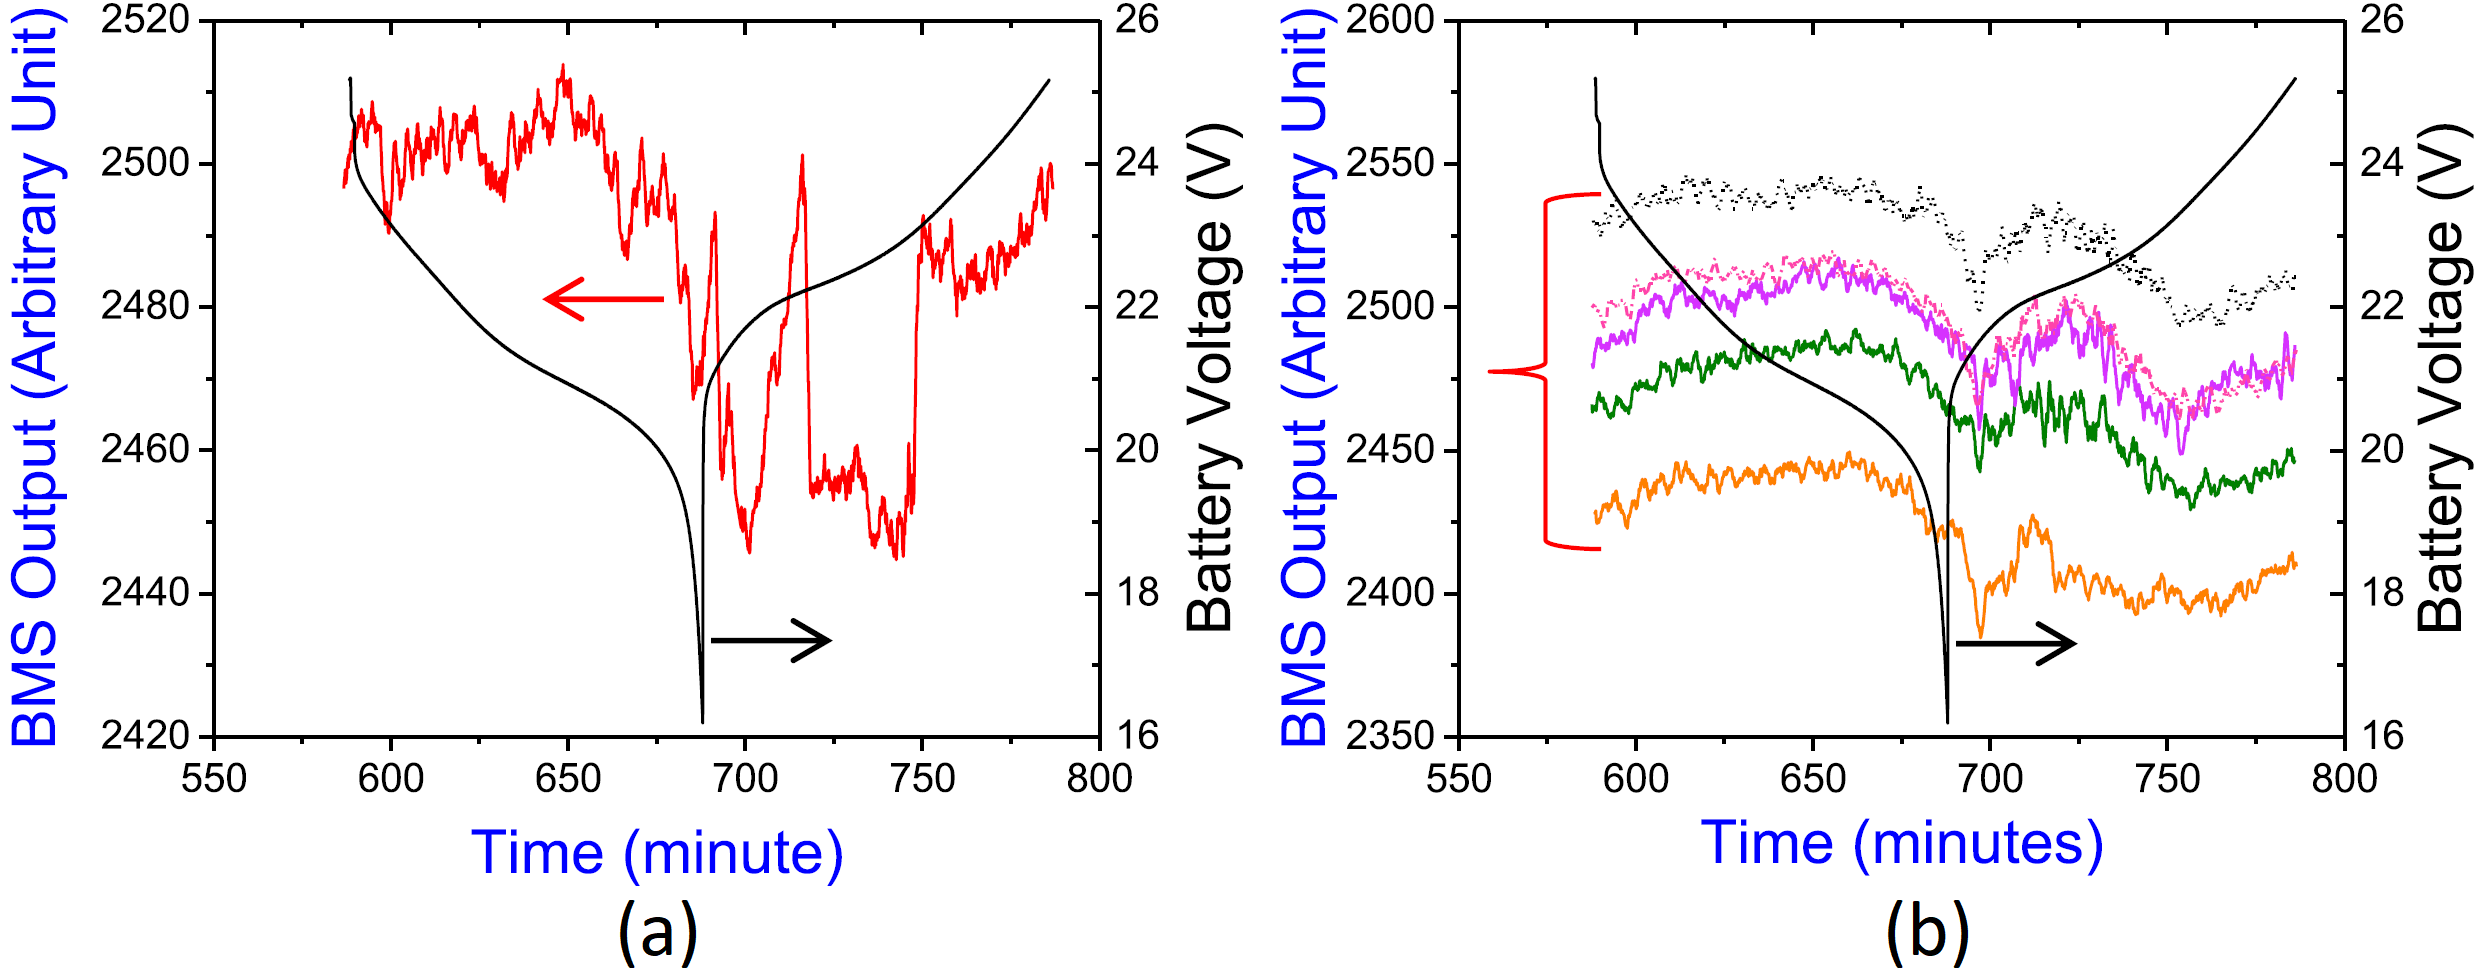
\includegraphics[width=16cm,height=6cm]{figures/result}
	\centering
	\caption{Outputs of impedance-based BITS-BMS for a six-cell battery containing five calendar-aged cells and one over-discharged cell, during a discharge–charge cycle: (a) Overdischarged cell only; (b) five calendar-aged, otherwise normal cells.} \label{result}
\end{figure}


	\chapter{Conclusion}

Conventional BMS monitor only $E_{cv}$ , $T_{surf}$ , and $R_s$ at a single frequency. They are not enough to ensure safety of the Li-ion battery. The tests showed that $E_{cv}$ , $T_{surf}$ and $R_s$ are not indicators for aging or overdischarge-induced cell mismatches. An impedance-based BITS-BMS, described here \cite{8247206}, that measures amplitude and phase shift at multiple frequencies can identify safety-relevant characteristics associated with anode, cathode, and electrolyte malfunction. Traditionally, such multifrequency BMS are large and require high electric power to operate, therefore have not spread. Portable BMS that measure impedance do so at a fixed single frequency. These single-frequency measurements are also limited to measuring either the real or quadrature (imaginary) component. A small-size, low power, standalone BMS that is enabled by multifrequency (1-1000 Hz) impedance meter that has phase and amplitude monitoring capability was shown in this paper. This BITS-BMS enables battery operation within a user-set range (internal temperature, cell voltage, etc.) and communicates with control systems to regulate charge and discharge currents. The BITS-BMS can identify cell mismatch, and ensure thermal safety and electrical efficiency in Li-ion batteries with multiple cells using simultaneous monitoring of $T_{int}$ , $E_{cv}$ and $R_s$ in each cell.	
\clearpage
	\addcontentsline{toc}{chapter}{References}
	\bibliographystyle{ieeetr}
	\bibliography{Report}
	\nocite{8247206}
	\nocite{dey2016sensor}
	\nocite{giegerich2016open}
	\nocite{taylor2012system}
	\nocite{osaka2015development}
	\nocite{waag2014critical}
\end{document}

